\chapter{KAJIAN PUSTAKA}


\section*{ }
Demi mendukung tutorial ini, dibutuhkan beberapa teori penunjang sebagai bahan acuan dan referensi. Dengan demikian tutorial ini menjadi lebih terarah. 
\vspace{1ex}

\section{Cara Menulis Daftar}
\underline{Menulis Dartar Item}
\begin{itemize}
	\item Ini Urutan Pertama. Ini Urutan Pertama. Ini Urutan Pertama. Ini Urutan Pertama. Ini Urutan Pertama. Ini Urutan Pertama. Ini Urutan Pertama. 
	\item Menulis Item kedua.Menulis Item kedua.Menulis Item kedua.Menulis Item kedua.Menulis Item kedua.Menulis Item kedua.Menulis Item kedua.
	\item Ini Urutan Ketiga
\end{itemize}

\underline{Menulis daftar urutan}
\begin{enumerate}
	\item Ini Urutan Pertama
	\item Ini Urutan kedua
	\begin{enumerate}
		\item Sub Urutan Pertama
		\item Sub Urutan Kedua
	\end{enumerate} 
	\item Ini Urutan Ketiga
\end{enumerate}


\section{Cara Penulisan Persamaan}
Cara menulis persamaan  inline pada text $\sum_{i=1}^{N} x_iy_i$


Contoh Integral
\begin{equation}\label{eq:persamaan1}
y=\int_{0}^{2\pi} cos(x) dx
\end{equation}
Persamaan \ref{eq:persamaan1} adalah contoh menulis fungsi $cos(\alpha x)$ dari $0\le x\le 2\pi$.\\
Menjajarkan persamaan
\begin{align}
y&=\int_{0}^{2\pi}cos(x)dx\\
&=sin(x)|_0^{2\pi}\\
&=sin(2\pi)-sin(0)\\
&=0
\end{align}
Persamaan \ref{eq:matrix} adalah matrix.
\begin{equation}\label{eq:matrix}
\textbf{X}=\begin{bmatrix}
x_{11}&x_{12}&\cdots&x_{1m}\\
x_{21}&x_{22}&\cdots&x_{2m}\\
\vdots&\vdots&\ddots&\vdots\\
x_{n1}&x_{n2}&\cdots&x_{nm}
\end{bmatrix}
\end{equation}
\vspace{1ex}
\section{Cara Penulisan Tabel}
\begin{table}[H]
	\caption{Tabel Contoh}
	\begin{tabular}{|l|l|l|l|}
		\hline
		No & X & Y & C \\ \hline
		1 & 0 & 0 & 1 \\ \hline
		2 & 0 & 1 & 0 \\ \hline
		3 & 1 & 0 & 0 \\ \hline
		4 & 1 & 1 & 0 \\ \hline
	\end{tabular}
\end{table}


\begin{table}[H]
	\label{tab:tabelcontoh2}
	\caption{Tabel ini contoh 2}
	\begin{tabular}{|l|l|l|l|}
		\hline
		\multirow{2}{*}{\textbf{No}} & \multicolumn{3}{l|}{\textbf{Data}} \\ \cline{2-4} 
		& \textbf{x} & \textbf{y} & \textbf{z} \\ \hline
		\textbf{1} & \textbf{0.1} & \textbf{0.2} & \textbf{0.3} \\ \hline
		\textbf{2} & \textbf{0.4} & \textbf{0.5} & \textbf{0.6} \\ \hline
	\end{tabular}
\end{table}
Pada Tabel \ref{tab:tabelcontoh2} di tunjukan cara membuat tabel.


\begin{sidewaystable}
	\centering
	\caption{Tabel ke samping}
	\begin{tabular}{|l|l|l|l|}
		\hline
		\multirow{2}{*}{\textbf{No}} & \multicolumn{3}{l|}{\textbf{Data}} \\ \cline{2-4} 
		& \textbf{x} & \textbf{y} & \textbf{z} \\ \hline
		\textbf{1} & \textbf{0.1} & \textbf{0.2} & \textbf{0.3} \\ \hline
		\textbf{2} & \textbf{0.4} & \textbf{0.5} & \textbf{0.6} \\ \hline
	\end{tabular}
	
\end{sidewaystable}
\newpage
\section{Cara Meletakan Gambar}
\begin{figure}[H]
	\centering
	
\includegraphics[width=0.5\linewidth]{bab2/LambangTeknikElektro}
	\caption{Lambang Teknik dengan Ukuran 0.5 Lebar Kertas}
	\label{fig:lambangteknikelektro}
\end{figure}
\begin{figure}[H]
	\centering
	
\includegraphics[width=0.2\linewidth]{bab2/LambangTeknikElektro}
	\caption{Lambang Teknik dengan Ukuran 0.2 lebar kertas}
	\label{fig:lambangteknikelektro2}
\end{figure}
\begin{figure}[H]
	\centering
	
\includegraphics[width=0.5\linewidth]{bab2/LambangTeknikKOmputer}
	\caption{Lambang Teknik Komputer  }
	\label{fig:lambangteknikkomputer}
\end{figure}
\section{Cara Membuat  sitasi}

Ini adalah cara  sitasi ke buku menggunakan cite\{Refferensi\}\\

Contoh : sitasi ke 1
 \cite{Brathwaite2009}.\\
Daftar referensi terletak pada file 
\textit{lainnya/pustaka.bib}\\

contoh  sitasi ke 2
\cite{Friedman1997}
\newline
\section{Algoritma}
Contoh Algoritma

\begin{algorithm}[H]
	\SetKwInOut{Input}{Input}
	\SetKwInOut{Output}{Output}
	
	\underline{function Euclid} $(a,b)$\;
	\Input{Two nonnegative integers $a$ and $b$}
	\Output{$\gcd(a,b)$}
	\eIf{$b=0$}
	{
		return $a$\;
	}
	{
		return Euclid$(b,a\mod b)$\;
	}
	\caption{Euclid's algorithm for finding the greatest common divisor of two nonnegative integers}
\end{algorithm}
\newpage
\section{Tools Online Yang Cukup Membantu}
Beberapa tools yang dapat digunakan untuk menulis tesis dengan latex.
\subsection{Online equation editor: HostMath }
\begin{center}
	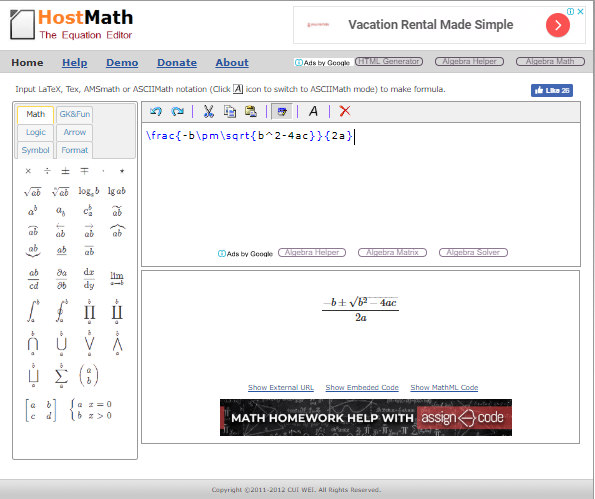
\includegraphics[width=1\linewidth]{bab2/Hosmath}
	\captionof{figure}{http://hostmath.com/}
	\label{fig:hosmath}
\end{center}




\newpage
\subsection{Detexify LaTeX handwritten symbol recognition}
\begin{center}
	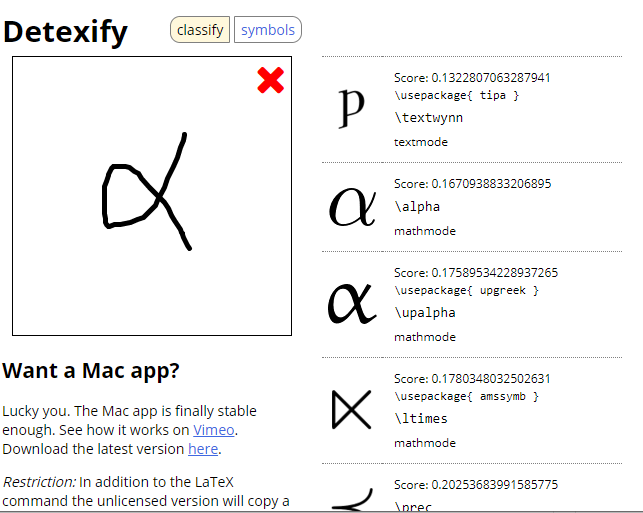
\includegraphics[width=\linewidth]{bab2/Detexify}
	\captionof{figure}{http://detexify.kirelabs.org/classify.html}
	\label{fig:detexify}
\end{center}
\newpage
\subsection{Tables Generator }
\begin{center}
	
	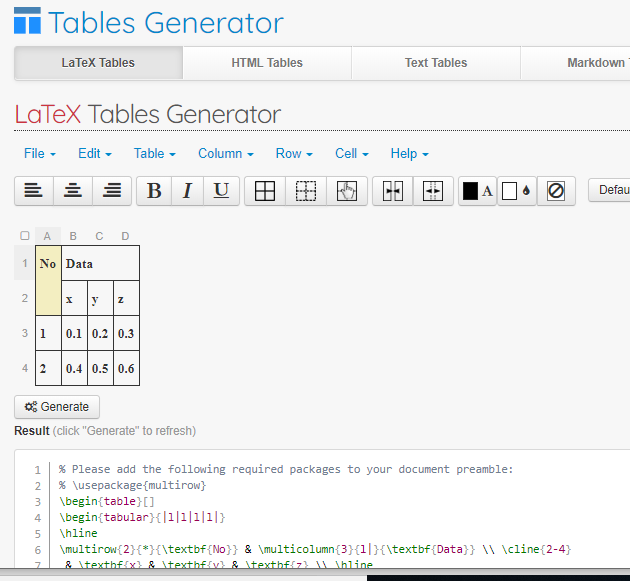
\includegraphics[width=0.7\linewidth]{bab2/TabelGenerator}
	\captionof{figure}{https://www.tablesgenerator.com/}
	\label{fig:tabelgenerator}
\end{center}

\subsection{Long Table}
\begin{landscape}

\begin{spacing}{1}	
\begin{longtable}{|p{3cm}| p{7cm} | p{7cm} | p{7cm}|}\label{table:Posisidankontribusipenelitian}\\
	\caption{Posisi dan kontribusi penelitian}\\
	%\toprule
	\hline
	\nohyphens{\textbf{Topik riset Registrasi}}  & \textbf{Metode}  &\nohyphens{\textbf{Kontribusi Peneliti Lain}}&\nohyphens{\textbf{Kontribusi Peneliti}} \\ 
	%\midrule
	\hline
	\endfirsthead
	\caption{Posisi dan kontribusi penelitian \textit{(Lanjutan..)}}\\
	%\toprule
	\hline
	
	\nohyphens{\textbf{Topik riset Registrasi}}  & \textbf{Metode}  &\nohyphens{\textbf{Kontribusi Peneliti Lain}}&\nohyphens{\textbf{Kontribusi Peneliti}} \\ 
	%\midrule
	\hline
	\endhead
	\multicolumn{4}{r}{{(\textit{Tabel bersambung..})}} \\
	\endfoot
	\endlastfoot 
	Ekstraksi feature& 	Kurvature  pada suatu titik di hitung pada beberapa skala dengan fitting  permukaan ke  titik lokal pada berbagai macam ukuran. (Ho dan Gibbins, 2009) & 	Multi-scale  Feature Extraction from 3D Meshes and Unstructured Point Cloud& \\ \hline 
	Estimasi vektor normal& 	Fitting tangen vektor pada  data titik untuk menentukan vektor normal berbasis local voronoy mesh. (OuYang dan Feng, 2005) & 	Metoda baru untuk estimasi vektor normal. & \\ \hline 
	Estimasi principal direction& 	The Adjacent-Normal Cubic Approximation 
	(Goldfeather dan Interrante, 2004) & 	Estimasi principal direction dan vektor normal pada permukaan dengan noise yang tinggi.&\\ \hline 
	Registrasi berbasis fitur permukaan. & 	Normal distribution transform.
	(Pathak, Birk,Vaskevicius dan Poppinga, 2010) & 	Online registrasi pose untuk menentukan posisi robot. & 	 \\ \hline 
	Registrasi 3D berbasis warna. & 	Warna rgb (Johnson dan Kang, 1997). 
	(Douadi dkk., 2006) & 	Menggantikan fitur geometri ketika informasi geometri permukaan tidak mencukupi. & 	\\ \hline 
	& 	Registrasi berbasis warnoHSV. (Druon, Aldon dan Crosinier, 2006) & 	Registrasi tidak di pengaruhi oleh intensitas warna. & 	\\ \hline 
	& 	Registrasi dengan Modified color ICP kombinasi antara warna RGB dengan jarak ecludiean.  (Joun,Ang,Kang,Chung dan Yu(2009) & 	Registrasi untuk lingkungan 3D. & 	\\ \hline 
	Registrasi Berbasis geometri permukaan.& 	Registrasi dengan angular invariant feature.  (Jiang dkk., 2009) & 	\textit{Angular  invariant feature} invariant terhadap rotasi dan skala. & 	\\ \hline 
	& 	Point  Feature Histograms (PFH)  robust multi-dimensional features. (Rusu, Blodow, Marton, Soos dan Beetz, 2007) & 	Kombinasi curvature, vektor normal dan vektor pcincipal direction. & 	\\ \hline 
	& 	Fitting quadratik surface  (Chen dan Bhanu, 2007) & 	Permukaan lokal sebagai deskriptor untuk Kombinasi curvature, vektor normal dan vektor pcincipal direction. & 	\\ \hline 
	& 	& 	& 	Registrasi Citra  2D multiview untuk penangkap gerak manusia
	Semina Sesindo 2010 (Yuniarno, Mardi, Sumpeno dan Hariadi, 2010)\\ \hline 
	& 	& 	& 	Registrasi permukaan berbeasis surface curvature feature.
	Jurnal Jatit  (Yuniarno, Hariadi dan Purnomo, 2013a) \\ \hline 
	Outlier Removal& 	Tiga konstrain untuk memperoleh korspondensi akurat. 
	(Liu, 2008)& 	Korespondensi yang akurat& 	\\ \hline 
	& 	Dua  konstrain untuk memperoleh korspondensi akurat. 
	(Xin dan Pu, 2010)& 	Perbaikan tiga konstrain yang diusulkan oleh Liu dengan meletakan origin ke titik berat permukaan.& 	\\ \hline 
	& 	& 	& 	perbaikan korespondensi 
	dengan rigid constraint berbasis dua titik referensi dan surface curvature feature Jurnal Kursor (Yuniarno, Hariadi dan Purnomo, 2013b)\cite{Brathwaite2009} \\ \hline 
\end{longtable}

\end{spacing}

\end{landscape}
\section{Tabel Rencana Penelitian }


\begin{table}[h!]
	\caption{Rencana Penelitian}
	\begin{tabular}{|l|l|l|l|l|l|l|l|l|l|}
		\hline
		& \multicolumn{9}{c|}{\textbf{Semester Ke}} \\ \cline{2-10} 
		\multirow{-2}{*}{} & 1 & 2 & 3 & 4 & 5 & 6 & 7 & 8 & 9 \\ \hline
		Rencana 1 & \cellcolor[HTML]{000000} & \cellcolor[HTML]{000000} & \cellcolor[HTML]{000000} & \cellcolor[HTML]{000000} & \cellcolor[HTML]{000000} &  &  &  &  \\ \hline
		Rencana 2 &  &  & \cellcolor[HTML]{000000} & \cellcolor[HTML]{000000} & \cellcolor[HTML]{000000} & \cellcolor[HTML]{000000} & \cellcolor[HTML]{000000} &  &  \\ \hline
		Rencana 3 &  &  &  &  &  & \cellcolor[HTML]{000000} & \cellcolor[HTML]{000000} & \cellcolor[HTML]{000000} & \cellcolor[HTML]{000000} \\ \hline
		Rencana 4 &  & \cellcolor[HTML]{000000} & \cellcolor[HTML]{000000}{\color[HTML]{000000} } & \cellcolor[HTML]{000000}{\color[HTML]{000000} } & \cellcolor[HTML]{000000}{\color[HTML]{000000} } & \cellcolor[HTML]{000000}{\color[HTML]{000000} } & \cellcolor[HTML]{000000}{\color[HTML]{000000} } & \cellcolor[HTML]{000000}{\color[HTML]{000000} } & \cellcolor[HTML]{000000}{\color[HTML]{000000} } \\ \hline
	\end{tabular}
\end{table}



